\subsection{Segel}
Das Segel besteht aus EPS und setzt sich aus vier identischen Teilen zusammen, die aus EPS-Platten ausgeschnitten werden. Je zwei Platten bilden die rechte und die linke Seite des Segels, das eine aerodynamisch günstige Form aufweist. Dazu werden die beiden Segelhälften verklebt.
\subsubsection*{EPS Schneidegerät}
Mit speziellen Schneidegeräten können Formen aus EPS Platten geschnitten werden. Konventionelle EPS Schneidegeräte sind allerdings nicht genügend gross, um die vier Teile auszuschneiden, weshalb ein eigenes Schneidegerät gebaut werden muss. Alle EPS-Schneidegeräte funktionieren nach demselben Prinzip. Dabei wird ein Metalldraht auf  60$^\circ$ C - 100$^\circ$ C erhitzt und ins EPS gefahren, wo dieses lokal zum Schmelzen gebracht wird. Indem der Draht durch den EPS Körper gezogen wird, entsteht ein sauberer Schnitt. Der Draht wird dadurch erhitzt, dass an ihm eine elektrische Spannung gelegt wird. Der Draht bildet einen Widerstand und wird heiss. Der Draht ist so ausgelegt, dass er einen möglichst hohen Widerstand aufweist. 
Damit die  vier grossen Segelteile als Ganzes aus EPS Blöcken geschnitten werden können, wird ein eigenes einfaches Schneidegerät mit entsprechenden Dimensionen gebaut.  Dazu wird ein sogenannter \enquote{Widerstandsdraht} mit einem Durchmesser von $\varnothing$ 0.2 mm gekauft. Dieser wird dreifach verdrillt und daraus ein Schneidedraht mit einer Länge von 1.5 m erstellt. Die beiden Enden werden in einen u-förmigen Rahmen aus Tannenholzlatten gespannt. Als Stromquelle dient zunächst ein Labornetzteil, das 3 A bei 12 V liefert. 

Die ersten Versuche, zunächst noch mit einem einfachen und anschliessend mit einem zweifachen Draht, verlaufen erfolglos. Erst als ein dreifach verdrillter Draht und ein stärkeres Labornetzteil, das 5 A bei 12 V liefert, verwendet wird, wird der Draht soweit aufgeheizt, dass damit EPS geschnitten werden kann.     
\begin{figure}[H]
    \centering
    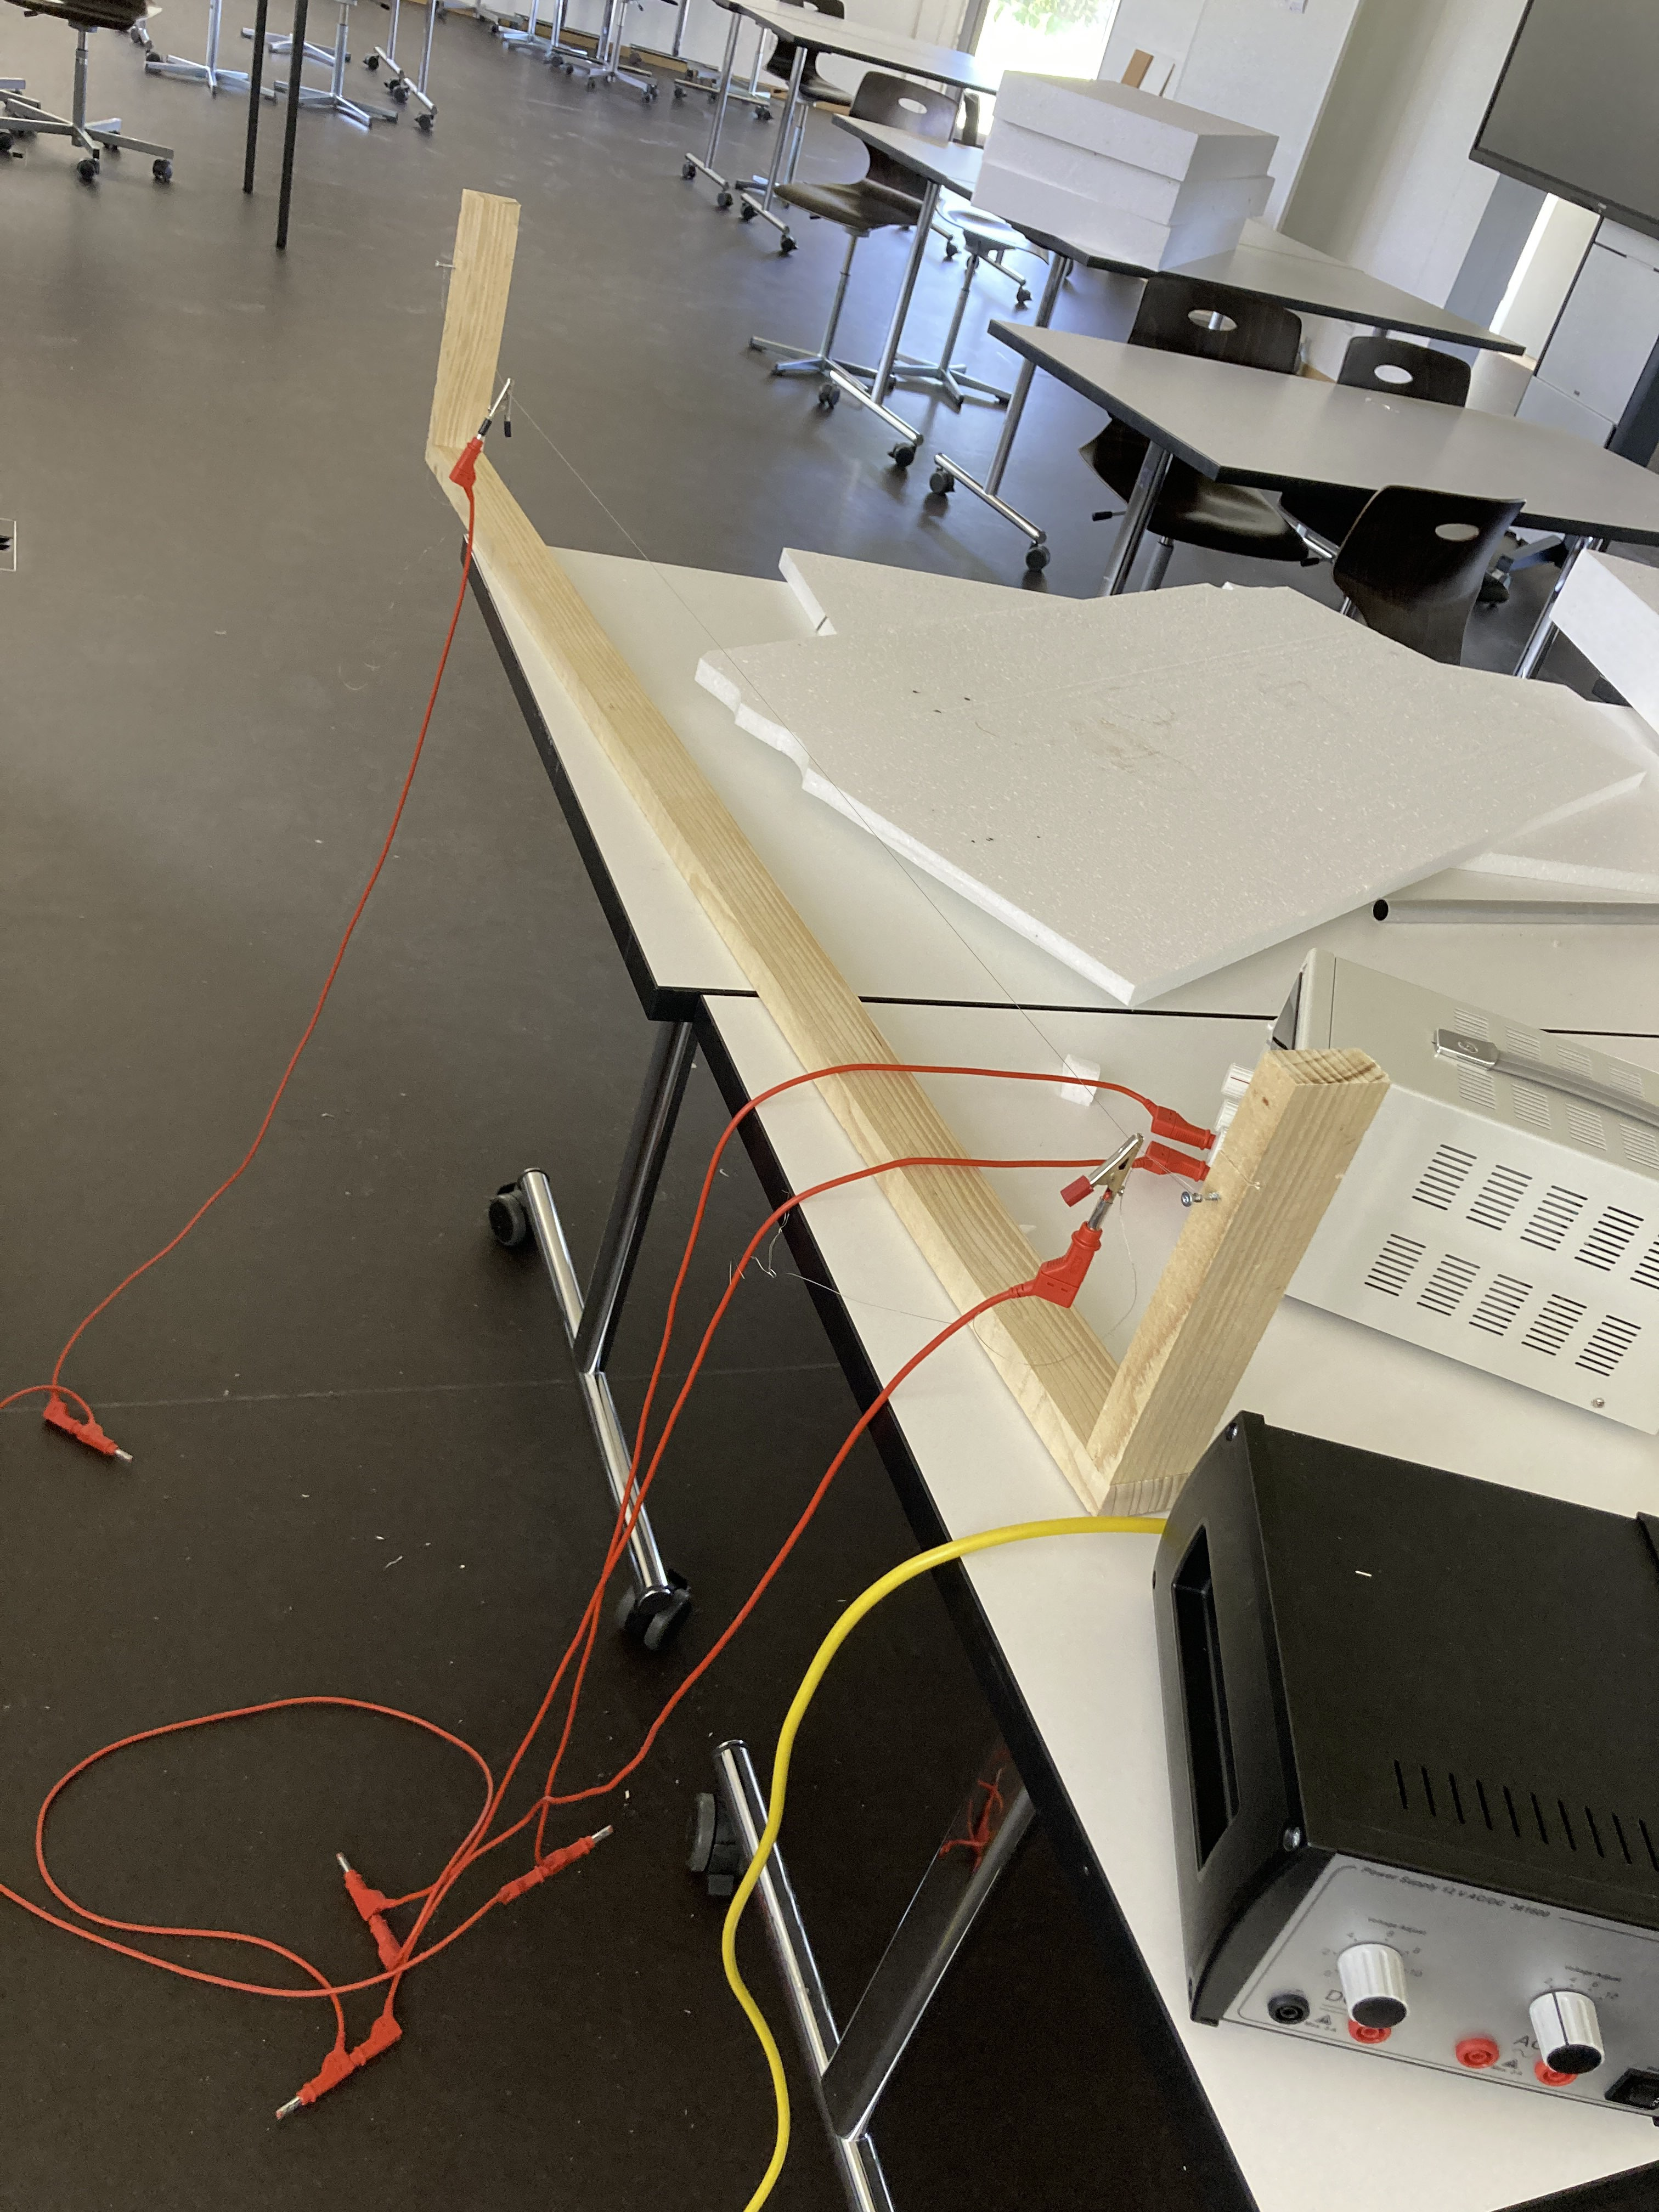
\includegraphics[width=0.5\linewidth]{foamcutter1.png}
    \caption{Foamcutter}
    \label{fig:enter-label}
\end{figure}
\subsection*{Grosssegel}
Um die geplante Form aus den \ac{eps} Platten schneiden zu können, wird zuerst mithilfe eines Lasercutters eine Halbprofilform aus Sperrholz erstellt. Je eine solche Halbprofilform wird mit zwei Schrauben an den beiden kürzeren Seiten einer EPS Platte  befestigt. Der heisse Schneidedraht kann damit entlang der Kante der Halbprofilschablone durch den EPS Block gezogen werden. So entsteht ein halbes Segel mit der Form der Halbprofilschablonen. \\


\begin{figure}[H]
    \centering
    \includegraphics[width=1\linewidth]{assets/template_on_foam.png}
    
    \caption{Seitenansicht eines Elements mit der Schablone}
    \label{fig:enter-label}
\end{figure}

Anschliessend muss auf der planen Seite des Halbsegelteils noch eine halbrunde Kerbe ausgeschnitten werden. In ihr findet bei der Verleimung der Platten der Aluminiummast Platz. Nicht jeder Schneideversuch verläuft erfolgreich. Wenn die beiden Enden des Schneiddrahtes nicht synchron über die Halbprofilform geführt werden oder wenn dieser nicht präzis gefolgt wird, weist der ausgeschnittene Körper erhebliche Formfehler auf. Auch bei einem an sich erfolgreichen Schnitt ergeben sich aber kleine Ungenauigkeiten, die aber mit einem Schliff des Bauteils korrigiert werden können. 

Nachdem erfolgreich vier Profile ausgeschnitten worden sind, wird der Mast in die ausgesparte Kerbe gelegt und fixiert. Danach werden die vier Profile in Paaren verklebt. Im Bootskörper sind zwei Halterungen für den Mast vorgesehen, die ein Kugellager enthalten. Der Mast wird durch deren Öffnungen gesteckt und am Schluss in den Schleifring gesteckt.
\subsection{Sailflap}
Das Sailflap wird mit derselben Technik wie das Grosssegel hergestellt. Zu seiner Befestigung werden zwei Carbonstäben verwendet, die am Grosssegel fixiert werden. Am unteren Stab wird der Aktuator befestigt, bevor das Sailflap mit den Carbonstäben fixiert wird. Zum Abschluss wird das Sailflap an der Welle des Aktuators befestigt.